% vim: set textwidth=78 autoindent:

\subsection{eVis Plugin}\label{sec:evis}

The Biodiversity Informatics Facility at the American Museum of Natural History's (AMNH) Center 
for Biodiversity and Conservation (CBC) \footnote{This section is derived from Horning, N., K.
Koy, P. Ersts. 2009. eVis (v1.1.0) User's Guide. American Museum of
Natural History, Center for Biodiversity and Conservation. Available from
\url{http://biodiversityinformatics.amnh.org/}, and released under the GNU FDL.} has developed the
Event Visualization Tool (eVis), 
another software tool to add to the suite of conservation monitoring and decision support tools 
for guiding protected area and landscape planning. This plugin enables users to easily link 
geocoded (i.e., referenced with latitude and longitude or X and Y coordinates) photographs, 
and other supporting documents, to vector data in QGIS.

eVis is now automatically installed and enabled in new versions of QGIS, and as with all plugins, 
it can be disabled and enabled using the Plugin Manager (See Section \ref{sec:managing_plugins}).

The eVis plugin is made up of three modules: the Database Connection tool, Event ID tool, and 
the Event Browser. These work together to allow viewing of geocoded photographs and other documents 
that are linked to features stored in vector files, databases, or spreadsheets.

\subsubsection{Event Browser}\label{evis_browser}

The Event Browser module provides the functionality to display geocoded photographs that are linked
to vector features displayed in the QGIS map window. Point data, for example, can be from a vector
file that can be input using QGIS or it can be from the result of a database query. The vector
feature must have attribute information associated with it to describe the location and name of the
file containing the photograph and, optionally, the compass direction the camera was pointed when
the image was acquired. Your vector layer must be loaded into QGIS before running the Event Browser.

\minisec{Launch the Event Browser module}\label{evis_launch_browser}

To launch the Event browser module either click on the \toolbtntwo{event_browser}{Event Browser}
icon or click on \mainmenuopt{Plugins} > \dropmenuopt{eVis} >
\dropmenuopt{eVis Event Browser}. This will open the Generic Event Browser window.

The Generic Event Browser window has three tabs displayed at the top of the window. The Display tab
is used to view the photograph and its associated attribute data. The Options tab provides a number
of settings that can be adjusted to control the behavior of the eVis plugin. Lastly, the Configure
External Applications tab is used to maintain a table of file extensions and their associated
application to allow eVis to display documents other than images.

\minisec{Understanding the Display window}\label{evis_display_window}

To see the Display window click on the \tab{Display} tab in the Generic Event Browser
window. The Display window is used to view geocoded photographs and their associated attribute data.

\begin{figure}[ht]
   \begin{center}
\caption{\label{evisdisplay}The \emph{eVis} display window \nixcaption}
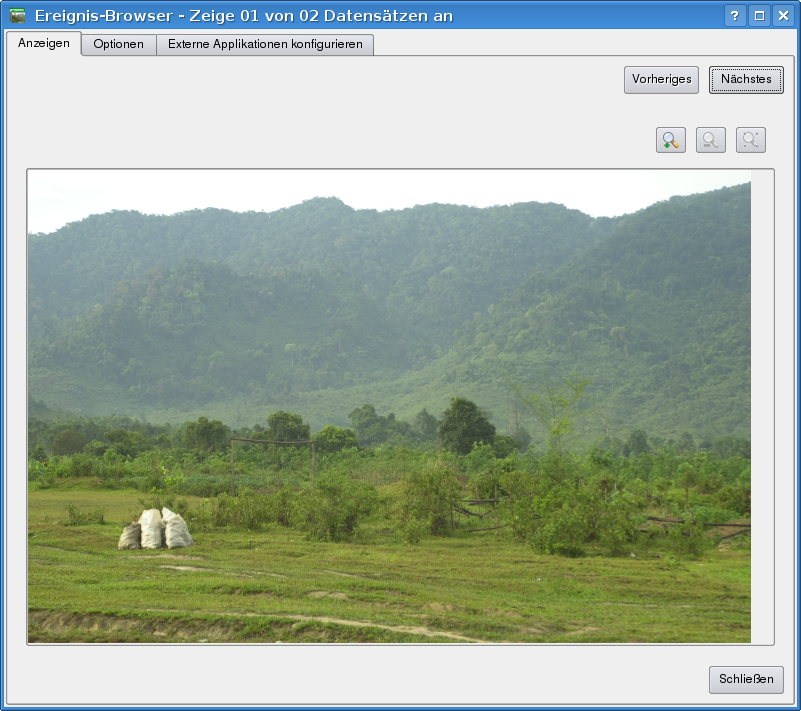
\includegraphics[clip=true, width=12cm]{evisdisplay}
\end{center}
\end{figure}

\begin{itemize}
\item \textbf{Display window}: A window where the photograph will appear.
\item \textbf{Increase zoom button}: Zoom in to see more detail. If the entire image cannot be
displayed in the display window, scroll bars will appear on the left and bottom sides of the window
to allow you to pan around the image.
\item \textbf{Reduce zoom button}: Zoom out to see more area. 
\item \textbf{Zoom to full extent button}: Displays the full extent of the photograph.
\item \textbf{Attribute information window}: All of the attribute information for the point
associated with the photograph being viewed is displayed here. If the file type being referenced in
the displayed record is not an image but is of a file type defined in the Configure External
Applications tab then when you double-click on the value of the field containing the path to the
file the application to open the file will be launched to view or hear the contents of the file. If
the file extension is recognized the attribute data will be displayed in green.
\item \textbf{Navigation buttons}: Use the Previous and Next buttons to load the previous or next
feature when more than one feature is selected.
\item \textbf{Feature indicator}: This heading indicates which feature is being displayed and how
many features are available for display.
\end{itemize}

\minisec{Understanding the Options window}\label{evis_options_window}

\begin{figure}[ht]
   \begin{center}
\caption{\label{evisoptions}The \emph{eVis} Options window \nixcaption}
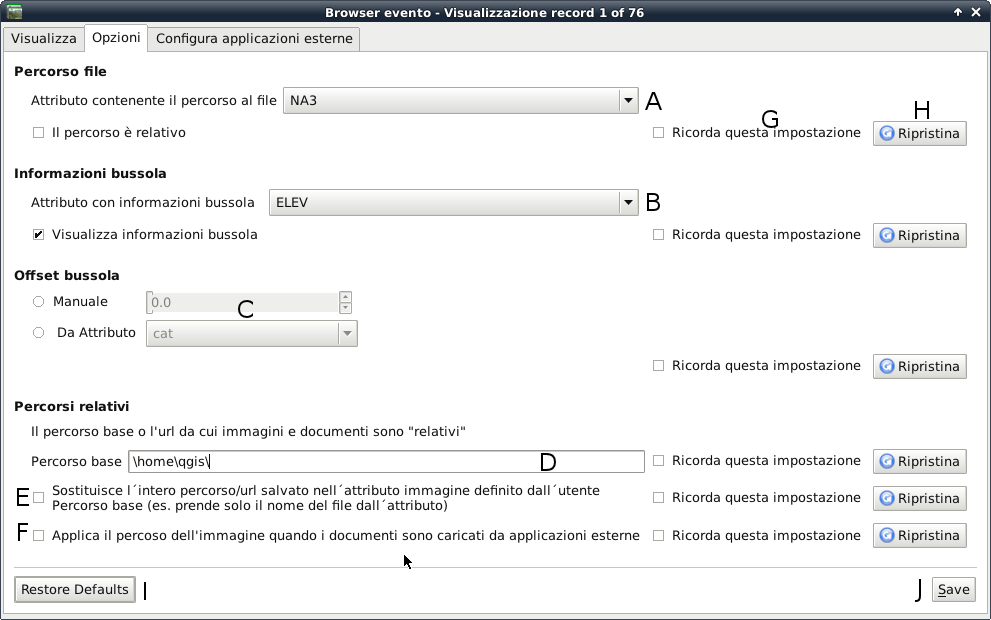
\includegraphics[clip=true, width=12cm]{evisoptions}
\end{center}
\end{figure}

\begin{itemize}
\item \textbf{File location}: A dropdown list to specify the attribute field that contains the
directory path or URL for the photographs or other documents being displayed. If the location is a
relative path then the checkbox to the right of the dropdown menu must be clicked. The base path for
a relative path can be entered in the Base Path text box below. Information about the different
options for specifying the file location are noted in the section 4.5 below.
\item \textbf{Compass bearing display field}: A dropdown list to specify the attribute field
that contains the compass bearing associated with the photograph being displayed. If compass bearing
information is available it is necessary to click the radio button to the left of the dropdown menu
title.
\item \textbf{Compass offset setting}: Compass offsets can be used to compensate for
declination (adjust bearings collected using magnetic bearings to true north bearings). Click the
Manual radio-button to enter the offset in the text box or click the From Attribute  radio-button to
select the attribute field containing the offsets. For both of these options east declinations
should be entered using positive values and west declinations should use negative values.
\item \textbf{Directory base path}: The base path onto which the relative path defined in
Figure \ref{evisoptions} (A) will be appended.
\item \textbf{Replace path}: If this check-box is checked, only the file name from the A
will be appended to the Base Path.
\item \textbf{Apply rule to all documents}: If checked, the same path rules that are defined
for photographs will be used for non-image documents such as movies, text documents, and sound
files. If not checked the path rules will only apply to photographs and other documents will ignore
the Base Path  parameter.
\item \textbf{Save settings}: If the check-box is checked the values for the associated
parameters will be saved for the next session when the window is closed or when the Save button
below is pressed.
\item \textbf{Reset values}: Resets the values on this line to the default setting.
\item \textbf{Restore faults}: This will reset all of the fields to their default settings.
It has the same effect as clicking all of the Reset buttons.
\item \textbf{Save}: This will save the settings without closing the Options pane.
\end{itemize}

\minisec{Understanding the Configure External Applications window}\label{evis_external_window}

\begin{figure}[htp]
   \begin{center}
\caption{\label{evisexternal}The \emph{eVis} External Applications window \nixcaption}
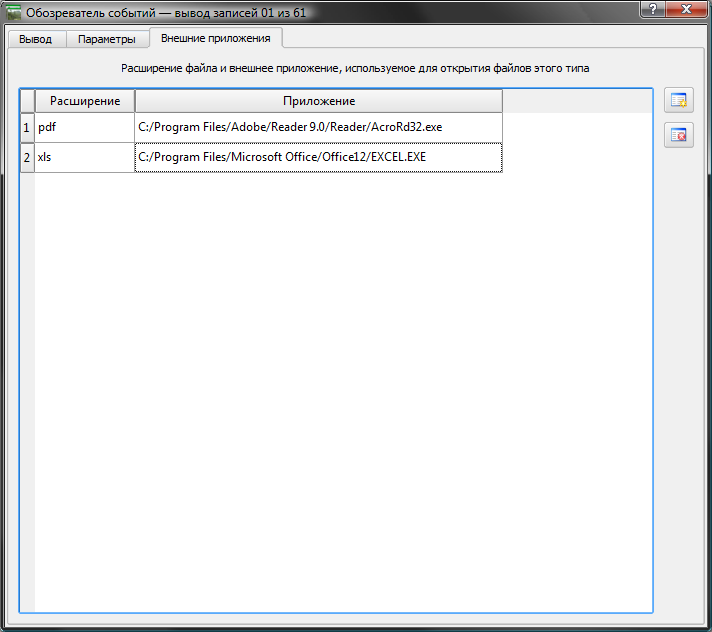
\includegraphics[clip=true, width=12cm]{evisexternal}
\end{center}
\end{figure}

\begin{itemize}
\item \textbf{File reference table}: A table containing file types that can be opened using eVis.
Each file type needs a file extension and the path to an application that can open that type of
file. This provides the capability of opening a broad range of files such as movies, sound
recordings, and text documents instead of only images.
\item \textbf{Add new file type}: Add a new file type with a unique extension and the path
for the application that can open the file.
\item \textbf{Delete current row}: Delete the file type highlighted in the table and defined
by a file extension and a path to an associated application.
\end{itemize}

\minisec{Specifying the location and name of a photograph}\label{evis_specifying}

The location and name of the photograph can be stored using an absolute or relative path or a URL if
the photograph is available on a web server. Examples of the different approaches are listed in
Table \ref{tab:evis_examples}.

\begin{table}[htp]\label{tab:evis_examples}\index{plugins!evis}
\centering
\caption{Example format using absolute path, relative path, and a
URL}\medskip
 \begin{tabular}{|p{0.55in}|p{0.55in}|p{4.7in}|p{0.7in}|}
 \hline \textbf{X} & \textbf{Y} & \textbf{FILE} & \textbf{BEARING}\\
 \hline 780596 & 1784017 & \filename{C:\textbackslash Workshop\textbackslash
eVis\_Data\textbackslash groundphotos\textbackslash DSC\_0168.JPG} & 275\\
 \hline 780596 & 1784017 & \filename{/groundphotos/DSC\_0169.JPG} & 80\\
 \hline 780819 & 1784015 &
\filename{http://biodiversityinformatics.amnh.org/evis\_test\_data/DSC\_0170.JPG} & 10\\
 \hline 780596 & 1784017 & \filename{pdf:http://www.testsite.com/attachments.php?attachment\_id-12}
& 76\\
 \hline
\end{tabular}
\end{table}

\minisec{Specifying the location and name of a other supporting
documents}\label{evis_location}

Supporting documents such as text documents, videos, and sound clips can also be displayed or played
by eVis. To do this it is necessary to add an entry in the file reference table that can be accessed
from the Configure External Applications window in the Generic Event Browser that matches the file
extension to an application that can be used to open the file. It is also necessary to have the path
or URL to the file in the attribute table for the vector layer. One
additional rule that can be used for URLs that don't contain a file extension for the document you
want to open is to specify the file extension before the URL. The format is - file extension:URL.
The URL is preceded by the file extension and a colon, and is particularly useful for accessing
documents from Wikis and other web sites that use a database to manage the web pages (see Table
\ref{tab:evis_examples}).

\minisec{Using the Generic Event Browser}\label{evis_using_browser}

When the Event Browser window opens a photograph will appear in the display window if the document
referenced in the vector file attribute table is an image and if the file location information in
the Options window is properly set. If a photograph is expected and it does not appear it will be
necessary to adjust the parameters in the Options window.

If a supporting document (or an image that does not have a file extension recognized by eVis) is
referenced in the attribute table the field containing the file path will be highlighted in green in
the attribute information window if that file extension is defined in the file reference table
located in the Configure External Applications window. To open the document double-click on the
green-highlighted line in the attribute information window. If a supporting document is referenced
in the attribute information window and the file path is not highlighted in green then it will be
necessary to add an entry for the file's filename extension in the Configure External Applications
window. If the file path is highlighted in green but does not open when double-clicked it will be
necessary to adjust the parameters in the Options window so the file can be located by eVis.

If no compass bearing is provided in the Options window a red asterisk will be displayed on top of
the vector feature that is associated with the photograph being displayed.
If a compass bearing is provided then an arrow will appear pointing in the direction indicated by
the value in the compass bearing display field in the Generic Event Browser window. The arrow will
be centered over the point that is associated with the photograph or other document.

To close the Generic Event Browser window click on the Close button from the Display window.

\subsubsection{Event ID Tool}\label{evis_id_tool}

The Event ID module allows you to display a photograph by clicking on a feature displayed in the
QGIS map window. The vector feature must have attribute information associated with it to describe
the location and name of the file containing the photograph and optionally the compass direction the
camera was pointed when the image was acquired. This layer must be loaded into QGIS before running
the Event ID tool.

\minisec{Launch the Event ID module}\label{evis_launch_id}

To launch the Event ID module either click on the \toolbtntwo{event_id}{Event ID}
icon or click on \mainmenuopt{Plugins} > \dropmenuopt{eVis} >
\dropmenuopt{Event ID Tool}. This will cause the cursor to change to an arrow with an``i'' on top of
it signifying that the ID tool is active.

To view the photographs linked to vector features in the active vector layer displayed in the QGIS
map window, move the Event ID cursor over the feature and then click the mouse. After clicking on
the feature, the Generic Event Browser window is opened and the photographs on or near the clicked
locality are available for display in the browser. If more than one photograph is available, you can
cycle through the different features using the Previous and Next buttons. The other controls are
described in the Event Browser section of this guide.

\subsubsection{Database connection}\label{evis_database}

The Database Connection module provides tools to connect to and query a database or other ODDBC
resource, such as a spreadsheet.

eVis can directly connect to four types of databases: Microsoft Access, PostgreSQL, MySQL, SQLITE,
and can also read from ODBC connections. When reading from an ODBC database (such as an Excel
spreadsheet) it is necessary to configure your ODBC driver for the operating system you are using.

\minisec{Launch the Database Connection module}\label{evis_launch_database}

To launch the Database Connection module either click on the appropriate icon
\toolbtntwo{evis_connect}{} or click on \mainmenuopt{Plugins} > \dropmenuopt{eVis} >
\dropmenuopt{Database Connection}. This will launch the Database Connection window. The window has
three tabs: \tab{Predefined Queries}, \tab{Database Connection}, and \tab{SQL Query}. The Output
Console window at the bottom of the window displays the status of actions initiated by the different
sections of this module.

\minisec{Connect to a database}\label{evis_connect_database}

Click on the \tab{Database Connection} tab to open the database connection interface. Next, click on
the \dropmenuopt{Database Type} dropdown menu to select the type of database that you want to
connect to. If a password or username is required, that information can be entered in the Username
and Password textboxes.

Enter the database host in the Database Host textbox. This option is not available if you selected
``MSAccess'' as the database type. If the database resides on your desktop you should enter
``localhost.''

Enter the name of the database in the Database Name textbox. If you selected ``ODBC'' as the
database type, you need to enter the data source name.

When all of the parameters are filled in, click on the Connect button. If the connection is
successful, a message will be written in the Output Console window stating that the connection was
established. If a connection was not established you will need to check that the correct parameters
were entered above.

\begin{figure}[ht]
   \begin{center}
\caption{\label{evisdatabase}The \emph{eVis} Database connection window \nixcaption}
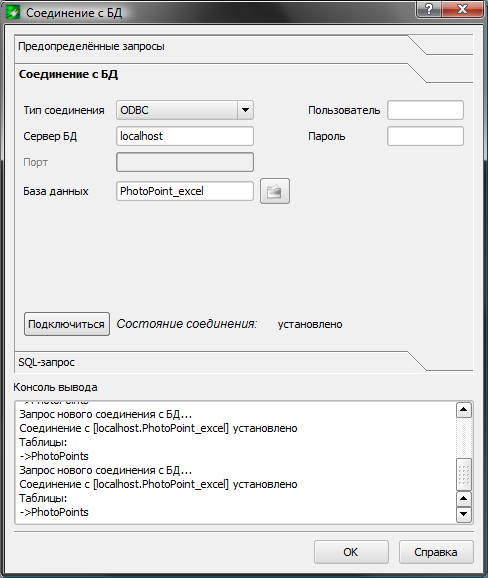
\includegraphics[clip=true, width=12cm]{evisdatabase}
\end{center}
\end{figure}

\begin{itemize}
\item \textbf{Database Type}: A dropdown list to specify the type of database that will be used.
\item \textbf{Database Host}: The name of the database host.
\item \textbf{Port} The port number if a ``MYSQL'' database type is selected.
\item \textbf{Database Name} The name of the database.
\item \textbf{Connect} A button to connect to the database using the parameters defined above.
\item \textbf{Output Console} The console window where messages related to processing are
displayed.
\item \textbf{Username}: Username for use when a database is password protected.
\item \textbf{Password}: Password for use when a database is password protected.
\item \textbf{Predefined Queries}: Tab to open the ``Predefined Queries'' window.
\item \textbf{Database Connection}: Tab to open the ``Database Connection'' window.
\item \textbf{SQL Query}: Tab to open the ``SQL Query'' window.
\item \textbf{Help}: Displays the on line help.
\item \textbf{OK}: Close the main ``Database Connection'' window.
\end{itemize}

\minisec{Running SQL queries}\label{evis_running_sql}

SQL queries are used to extract information from a database or ODBC resource. In eVis the output
from these queries is a vector layer added to the QGIS map window. Click on the \tab{SQL Query} tab
to display the SQL query interface. SQL commands can be entered in this text window. A helpful
tutorial on SQL commands is available at \url{http://www.w3schools.com/sql/}. For example, to
extract all of the data from a worksheet in an Excel file, ``select * from [sheet1\$]''
where``sheet1'' is the name of the worksheet.

Click on the Run Query button to execute the command. If the query is successful a Database File
Selection window will be displayed. If the query is not successful an error message will appear in
the Output Console widow.

In the Database File Selection window, enter the name of the layer that will be created from the
results of the query in the Name of New Layer textbox.

\begin{figure}[ht]
   \begin{center}
\caption{\label{evissql_query}The \emph{eVis} SQL query tab \nixcaption}
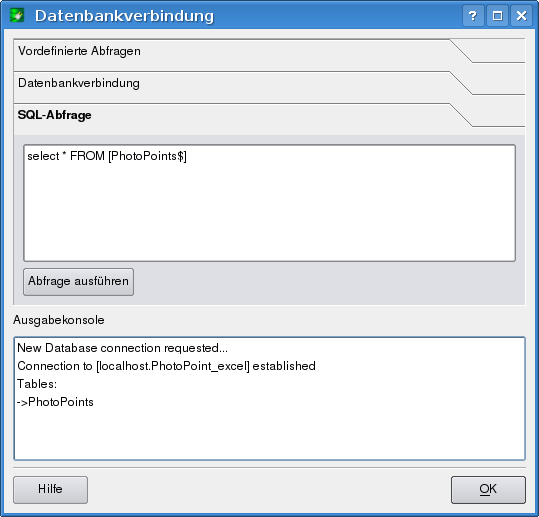
\includegraphics[clip=true, width=12cm]{evissql_query}
\end{center}
\end{figure}

\begin{itemize}
\item \textbf{SQL Query Text Window}: A screen to type SQL queries.
\item \textbf{Run Query}: Button to execute the query entered in the SQL Query Window.
\item \textbf{Console Window}: The console window where messages related to processing are
displayed.
\item \textbf{Help}: Displays the on line help.
\item \textbf{OK}: If this check-box is checked, only the file name from the A will be appended to
the Base Path.
\item \textbf{Apply rule to all documents}: Closes the main ``Database Connection'' window.
\end{itemize}

Use the \dropmenuopt{X Coordinate} and \dropmenuopt{Y Coordinate} dropdown menus to select the field
from the database that store the ``X'' (or longitude) and ``Y'' (or latitude) coordinates. Clicking
on the OK button causes the vector layer created from the SQL query to be displayed in the QGIS map
window.

To save this vector file for future use, you can use the QGIS ``Save as shapefile'' command that is
accessed by right clicking on the layer name in the QGIS map legend and then selecting ``Save as
shapefile.''

\begin{Tip}\caption{\textsc{Creating a vector layer from a Microsoft Excel Worksheet}}
\qgistip{When creating a vector layer from a Microsoft Excel Worksheet you might see that unwanted
zeros (``0'') have been inserted in the attribute table rows beneath valid data.This can be caused
by deleting the values for these cells in Excel using the ``backspace'' key. To correct this problem
you need to open the Excel file (you'll need to close QGIS if there if you are connected to the file
to allow you to edit the file) and then use Edit > Delete to remove the blank rows from the file. To
avoid this problem you can simply delete several rows in the Excel Worksheet using Edit > Delete
before saving the file.}
\end{Tip}

\minisec{Running predefined queries}\label{evis_predefined}

With predefined queries you can select previously written queries stored in XML format in a file.
This is particularly helpful if you are not familiar with SQL commands. Click on the \tab{Predefined
Queries} tab to display the predefined query interface.

To load a set of predefined queries click on the \toolbtntwo{evis_file}{Open File} icon. This opens
the Open File window which is used to locate the file containing the SQL queries. When the queries
are loaded their titles, as defined in the XML file, will appear in the dropdown menu located just
below the \toolbtntwo{evis_file}{Open File} icon, the full description of the query is displayed in
the text window under the dropdown menu.

Select the query you want to run from the dropdown menu and then click on the SQL Query tab to see
that the query has been loaded into the query window. If it is the first time you are running a
predefined query or are switching databases, you need to be sure to connect to the database.

Click on the \button{Run Query} button in the \tab{SQL Query} tab to execute the command. If the
query is successful a Database File Selection window will be displayed. If the query is not
successful an error message will appear in the Output Console window.

\begin{figure}[htp]
   \begin{center}
\caption{\label{evispredefined}The \emph{eVis} Perdefined queries tab \nixcaption}
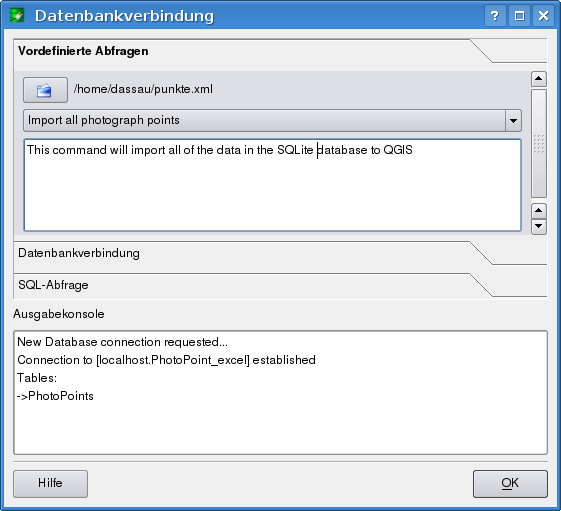
\includegraphics[clip=true, width=10cm]{evispredefined}
\end{center}
\end{figure}

\begin{itemize}
\item \textbf{Open Query File}: Launches the ``Open File'' file browser to search for the XML file
holding the predefined queries.
\item \textbf{Predefined Queries}: A dropdown list with all of the queries defined by the
predefined queries XML file.
\item \textbf{Query description}: A short description of the query. This description is from the
predefined queries XML file.
\item \textbf{Console Window}: The console window where messages related to processing are
displayed.
\item \textbf{Help}: Displays the on line help.
\item \textbf{OK}: Closes the main ``Database Connection'' window.
\end{itemize}

\minisec{XML format for eVis predefined queries}\label{evis_xml_format}

\begin{table}[htp]\index{plugins!evis}
\centering
\caption{The XML tags read by eVis}\label{tab:evis_xml_tags}\medskip
 \begin{tabular}{|p{1.2in}|p{4.7in}|}
 \hline \textbf{Tag} & \textbf{Description}\\
 \hline query & Defines the beginning and end of a query statement.\\
 \hline shortdescription & A short description of the query that appears in the eVis dropdown
menu.\\
 \hline description & A more detailed description of the query displayed in the Predefined Query
text window.\\
 \hline databasetype & The database type as defined in the Database Type dropdown menu in the
Database Connection tab.\\
 \hline databaseport & The port as defined in the Port textbox in the Database Connection tab.\\
 \hline databasename & The database name as defined in the Database Name textbox in the Database
Connection tab.\\
 \hline databaseusername & The database username as defined in the Username textbox in the Database
Connection tab.\\
 \hline databasepassword & The database password as defined in the Password textbox in the Database
Connection tab.\\
 \hline sqlstatement & The SQL command.\\
 \hline autoconnect & A flag (``true'' or ``false'') to specify if the above tags should be used to
automatically connect to database without running the database connection routine in the Database
Connection tab.\\
 \hline
\end{tabular}
\end{table}

A complete sample XML file with three queries is displayed below:

\begin{verbatim}
<?xml version="1.0"?>
<doc>
 <query>
   <shortdescription>Import all photograph points</shortdescription>
   <description>This command will import all of the data in the SQLite database to QGIS
      </description>
   <databasetype>SQLITE</databasetype>
   <databasehost />
   <databaseport />
   <databasename>C:\textbackslash Workshop/textbackslash
eVis\_Data\textbackslash PhotoPoints.db</databasename>
   <databaseusername />
   <databasepassword />
   <sqlstatement>SELECT Attributes.*, Points.x, Points.y FROM Attributes LEFT JOIN 
      Points ON Points.rec_id=Attributes.point_ID</sqlstatement>
   <autoconnect>false</autoconnect>
 </query>
  <query>
   <shortdescription>Import photograph points "looking across Valley"</shortdescription>
   <description>This command will import only points that have photographs "looking across 
      a valley" to QGIS</description>
   <databasetype>SQLITE</databasetype>
   <databasehost />
   <databaseport />
   <databasename>C:\Workshop\eVis_Data\PhotoPoints.db</databasename>
   <databaseusername />
   <databasepassword />
   <sqlstatement>SELECT Attributes.*, Points.x, Points.y FROM Attributes LEFT JOIN 
      Points ON Points.rec_id=Attributes.point_ID where COMMENTS='Looking across 
      valley'</sqlstatement>
   <autoconnect>false</autoconnect>
 </query>
 <query>
   <shortdescription>Import photograph points that mention "limestone"</shortdescription>
   <description>This command will import only points that have photographs that mention 
      "limestone" to QGIS</description>
   <databasetype>SQLITE</databasetype>
   <databasehost />
   <databaseport />
   <databasename>C:\Workshop\eVis_Data\PhotoPoints.db</databasename>
   <databaseusername />
   <databasepassword />
   <sqlstatement>SELECT Attributes.*, Points.x, Points.y FROM Attributes LEFT JOIN 
      Points ON Points.rec_id=Attributes.point_ID where COMMENTS like '%limestone%'
      </sqlstatement>
   <autoconnect>false</autoconnect>
 </query>
</doc>
\end{verbatim}
